\documentclass[]{article}

\usepackage{graphicx}
\usepackage{amsmath}
\usepackage{tikz}

%opening
\title{Support Vector Machines}
\author{Carmel Gafa}

\begin{document}

\maketitle

\begin{abstract}
This paper is the first in a series of articles that illustrate various algorithms that can be used in budget prediction scenarios. The objectives of these articles is to provide the necessary background and implementation knowledge to the persons involved in these challenges. It is the aim of these papers to be as exhaustive as possible; the required mathematical, implementation and practical issues are all discussed in length.
\end{abstract}

\section{Introduction}
In this first article, prediction based on support vector machines is investigated. Although support vector machines is widely known as a classification algorithm, as we shall see late on, it can be easily adapted top predict the most likely outcome in a series. 
TODO: history This paper is divided into XXXXXX
sections. First, the required mathematical concepts are discussed so to provide the necessary tools to examine support vector machines. A description of the concepts making up state vector machines can be found in Section \ref{sec:svm}.
TODO: other sections


\section{Mathematical Background}
The concepts necessary to understand the support vector machines algorithm in detail are discussed here so they can serve as a reference in the latter sections.

\subsection{Maximum and minimum values of a function of two variables}

A function $z = f(x,y)$ is said to have a maximum value at $P(a,b)$ if $f(a,b)$ is greater than the value at the near-by point $Q(a+\delta x, b+\delta y)$ for all values of $\delta x$ and $\delta y$ however small, positive or negative, that is in all directions from P.

Similarly,  $z = f(x,y)$ is said to have a minimum value at $P(a,b)$ is $f(a,b)$ is less than the value at the near-by point $Q(a+\delta x, b+\delta y)$ for all values of $\delta x$ and $\delta y$ however small, positive or negative, that is in all directions from P.

To determine minimum and maximum values we must therefore investigate the sign of the value of $f(a+\delta x, b+\delta y) - f(a,b)$
\bigskip

If $f(a+\delta x, b+\delta y) - f(a,b) < 0$ then we have a maximum value at $P(a,b)$

If $f(a+\delta x, b+\delta y) - f(a,b) > 0$ then we have a minimum value at $P(a,b)$

\bigskip
Now Taylor's theorem expands a function of two variables $f(x+ \delta x, y+\delta y)$ in terms of $f(x,y)$, powers of $ \delta x$ and $\delta y$ and successive derivatives of $f(x, y)$ and can be stated as

\begin{equation}
f(x+ \delta x, y+\delta y) = f(x, y) + \left\lbrace  \delta x f'_x(x,y) +\delta y f'_y(x,y) \right\rbrace  +  \frac{1}{2!} \left\lbrace  \delta x^{2}f''_{xx}(x,y)+ 2 \delta x \delta y f''_{yx}(x,y) +\delta y^{2}f''_{yy}(x,y) \right\rbrace + \dots
\end{equation}

Hence, in the case examined here, 

\[
f(a+ \delta x, b+\delta y) = f(a, b) + \left\lbrace  \delta x \frac{\partial f}{\partial x} +\delta y \frac{\partial f}{\partial y} \right\rbrace  + \frac{1}{2!} \left\lbrace  \delta x^{2}\frac{\partial^2 f}{\partial x^2}+ 2\delta x \delta y \frac{\partial^2 f}{\partial x\partial y} +\delta y^{2}\frac{\partial^2 f}{\partial y^2} \right\rbrace + \dots
\]

therefore, 

\[
f(a+\delta x, b+\delta y) - f(a, b) = \left\lbrace \delta x \frac{\partial f}{\partial x} +\delta y \frac{\partial f}{\partial y} \right\rbrace  + \frac{1}{2!} \left\lbrace \delta x^{2}\frac{\partial^2 f}{\partial x^2}+ 2\delta x \delta y \frac{\partial^2 f}{\partial x\partial y} +\delta y^{2}\frac{\partial^2 f}{\partial y^2} \right\rbrace + \dots
\]

For very small $\delta x$ and $\delta y$ higher order derivatives become negligible and the equation can be approximated by:


\[
f(a+\delta x, b+\delta y) - f(a, b) = \left\lbrace \delta x \frac{\partial f}{\partial x} +\delta y\frac{\partial f}{\partial y} \right\rbrace 
\]

For a stationary value of z at $(a,b)$

\[
f(a+\delta x, b+\delta y) - f(a, b) = \left\lbrace \delta x \frac{\partial f}{\partial x} +\delta y\frac{\partial f}{\partial y} \right\rbrace = 0
\]

Since $\delta x$ and $\delta y$ are small independent increments,

\[
\delta x \frac{\partial f}{\partial x} = 0 
\]
and
\[
\delta y\frac{\partial f}{\partial y} = 0
\]

\subsection{Lagrange Multipliers}

In many practical situations it is often required to determine the points at which stationary values occur, with the added condition that the points lie on a pre-described curve. This is referred to as a constrained optimization problem. In essence, the objective of this technique is to maximize (or minimize) some multivariate function that is however subject to a certain constraint. 

\begin{figure}[h]
\centering
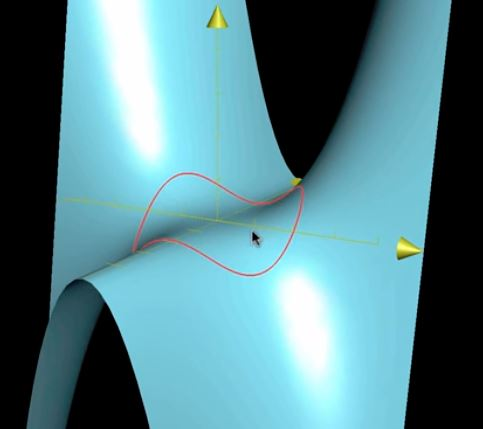
\includegraphics[width=0.7\linewidth]{img/fig_1}
\caption{A multivariate function subject to a constraint}
\label{fig:fig1}
\end{figure}

Figure \ref{fig:fig1} shows, as an example the function $f(x,y) = x^2 y$ subject yo a unit circle constraint $x^2 + y^2 = 1$. We notice that the projection of the circle on the function has a number of peaks (and troughs) and this techniques is used to determine the maximum peak. An alternative way to visualize this  function is to consider the x-y plane as in Figure \ref{fig:fig2} and visualize contour lines for the  $f(x,y)$, whilst clearly visualizing the constraint as the unit circle. Different values of $f(x,y)$ will produce different contours, some will intersect the constraint, others will lie outside. Of interest here is the contour that is tangent to the constraint as that is the maximum value of $f(x,y)$ given the stated constraint.

\begin{figure}[h]
\centering
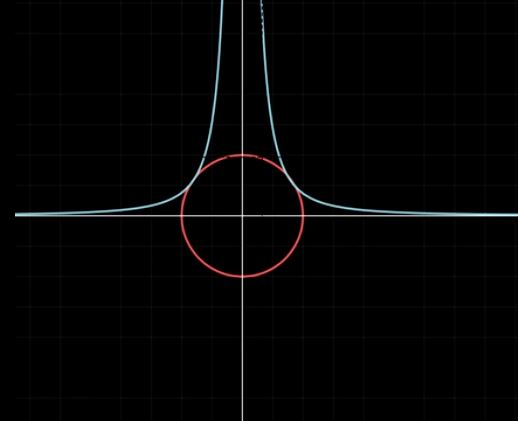
\includegraphics[width=0.7\linewidth]{img/fig_2}
\caption{X-Y plane projection of the system in Figure \ref{fig:fig1}}
\label{fig:fig2}
\end{figure}

\bigskip

So,if we, as an example, have to determine stationary points of the function

\[
f(x,y)
\]

with variables x and y constrained by the relation

\begin{equation}
\label{eqn:constraint}
\phi(x,y) = 0
\end{equation}

As we saw in the previous section the total differential reduced to zero at the stationary points, 

\begin{equation}
\label{eqn:u_zero}
\frac{\partial f}{\partial x} \delta x  +\frac{\partial f}{\partial y} \delta y  = 0
\end{equation}

Also, since $\phi(x,y) = 0$

\begin{equation}
 \label{eqn:phi_zero}
  \frac{\partial \phi}{\partial x} \delta x  +\frac{\partial \phi}{\partial y} \delta y  = 0
\end{equation}

if we multiply each term in (\ref{eqn:phi_zero}) be a multiplier $-\lambda$ and then add (\ref{eqn:phi_zero}) and (\ref{eqn:u_zero}) we get

\[
\left( \frac{\partial f}{\partial x} - \lambda \frac{\partial \phi}{\partial x} \right) \delta x  + 
\left( \frac{\partial f}{\partial y} - \lambda \frac{\partial \phi}{\partial y} \right) \delta y
 = 0
\]

since $ \delta x$ and  $\delta y$ are independent increments.

\begin{equation}
\frac{\partial f}{\partial x} - \lambda \frac{\partial \phi}{\partial x} = 0
\end{equation}

\begin{equation}
\frac{\partial f}{\partial y} - \lambda \frac{\partial \phi}{\partial y} = 0
\end{equation}

or 

\begin{equation}
\label{eqn:lang_f_x}
\frac{\partial f}{\partial x} = \lambda \frac{\partial \phi}{\partial x}
\end{equation}

\begin{equation}
\label{eqn:lang_f_y}
\frac{\partial f}{\partial y} = \lambda \frac{\partial \phi}{\partial y}
\end{equation}

or in matrix form

\[
\begin{bmatrix}
\frac{\partial f}{\partial x}\\ \\
\frac{\partial f}{\partial y}
\end{bmatrix}
=
\lambda
\begin{bmatrix}
\frac{\partial \phi}{\partial x}\\ \\
\frac{\partial \phi}{\partial y}
\end{bmatrix}
\]

These two equations together with the constraint equation (\ref{eqn:constraint}) that can be used to determine the values of x and y at the stationary points and if required, the value of $\lambda$.

Graphically this means, that at the maximum point, the gradient of $f(x_m,y_m)$ is proportional to the gradient of $\phi(x_m,y_m)$ and the constant of proportionality is the Lagrange multiplier $\lambda$, hence,
\begin{equation}
\label{eqn:lagrange_multiplier}
\bigtriangledown f(x_m,y_m) = \lambda \bigtriangledown  \phi(x_m,y_m)
\end{equation}

In the contour plot, the gradient at any point is perpendicular to the function, hence one can visualize equation (\ref{eqn:lagrange_multiplier}) in Figure \ref{fig:fig3}

\begin{figure}[h]
\centering
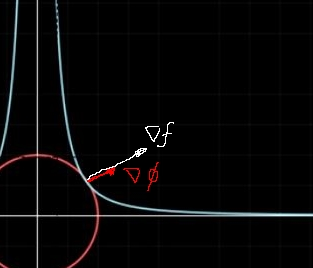
\includegraphics[width=0.7\linewidth]{img/fig_3}
\caption{Graphical representation of the Lagrange multiplier}
\label{fig:fig3}
\end{figure}

\subsection{The Lagrangian}

As we have seen previously, given a function to be maximized $f(x,y)$  constrained by $\phi(x,y)= b$, the maximum will be achieved when the contour of f is just tangent to that of $\phi$. Therefore the gradient of f, $\bigtriangledown f$ is proportional to that of $\phi$, $\bigtriangledown \phi$. The two gradients can be equated by the introduction of the Lagrange multiplier, 

\begin{equation}
\bigtriangledown f(x,y) = \lambda \bigtriangledown  \phi(x,y)
\end{equation}

The Lagrangian is defined as:

\begin{equation}
\mathcal{L}(x,y,\lambda) = f(x,y) - \lambda \left( \phi(x,y) - b \right) 
\end{equation}

where b is a constant.

Of particular importance is the value of $\bigtriangledown \mathcal{L} = \textbf{0}$ as

\[
\renewcommand\arraystretch{2}
\begin{bmatrix}
\frac{\delta \mathcal{L}}{\delta x} \\
\frac{\delta \mathcal{L}}{\delta y} \\
\frac{\delta \mathcal{L}}{\delta \lambda} \\
\end{bmatrix}
=
\begin{bmatrix}
0 \\
0 \\
0 \\
\end{bmatrix}
\]

If we consider
\[
\frac{\delta \mathcal{L}}{\delta x} = 0 
\]
 This can be evaluated to

\[
\frac{\delta f}{\delta x} -\lambda\left( \frac{\delta \phi}{\delta x}  \right)   = 0 
\]
or
\[
\frac{\delta f}{\delta x}  = \lambda\left( \frac{\delta \phi}{\delta x}  \right)
\]

which is equation (\ref{eqn:lang_f_x}). Similarly

\[
\frac{\delta \mathcal{L}}{\delta y} = 0 
\]
 can be evaluated to

\[
\frac{\delta f}{\delta y} -\lambda\left( \frac{\delta \phi}{\delta y}  \right)   = 0 
\]
or
\[
\frac{\delta f}{\delta y}  = \lambda\left( \frac{\delta \phi}{\delta y}  \right)
\]

which is equation (\ref{eqn:lang_f_y}).

Finally, 

\[
\frac{\delta \mathcal{L}}{\delta \lambda} = 0 
\]

 can be evaluated to

\[
-\left( \phi(x,y) - b\right)   = 0 
\]
or
\[
\phi(x,y) = b 
\]

which is the constraint equation.


\section{Support Vector Machines}
\label{sec:svm}

Decision boundary techniques separate data points into regions, or classes to which they belong.




\begin{figure}[h]
	\centering
	\usetikzlibrary{arrows}
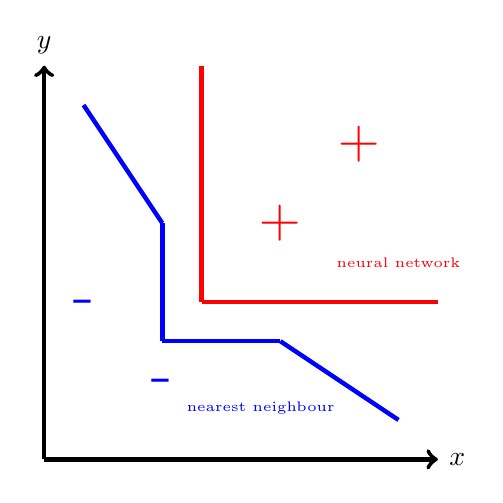
\begin{tikzpicture}


\draw[->,ultra thick] (0,0)--(5,0) node[right]{$x$};
\draw[->,ultra thick] (0,0)--(0,5) node[above]{$y$};

\node [text=blue] at (1.5,1) {\Huge -};
\node [text=blue] at (0.5,2) {\Huge -};
\node [text=red] at (3,3) {\huge +};
\node [text=red] at (4,4) {\huge +};

\draw[red,ultra thick] (2,5)--(2,2);
\draw[red,ultra thick] (5,2)--(2,2);


\draw[blue,ultra thick] (0.5,4.5)--(1.5,3);
\draw[blue,ultra thick] (1.5,3)--(1.5,1.5);
\draw[blue,ultra thick] (1.5,1.5)--(3,1.5);
\draw[blue,ultra thick] (3,1.5)--(4.5,0.5);

\node[red] at (4.5,2.5) {\tiny neural network};
\node[blue] at (2.75,0.65) {\tiny nearest neighbour};

\end{tikzpicture}+
	\caption{Different decision boundary techniques}
	\label{fig:fig4}
\end{figure}


The claim of support vector machines is that given a space with negative samples and positive samples a divisor can be constructed with the view towards putting in the widest boundary that separates the positive samples from the negative ones; thus maximizing the separation between the classes.

\begin{figure}[h]
	\centering
	\usetikzlibrary{arrows}
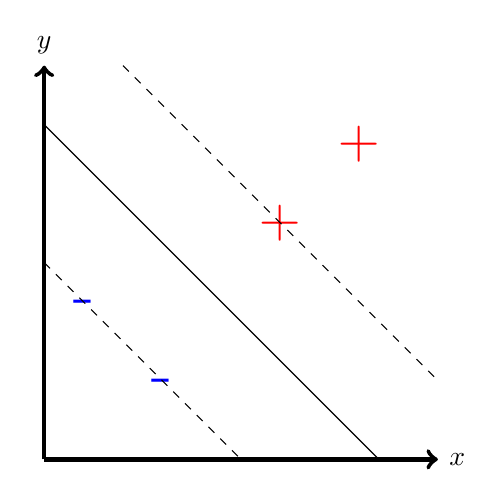
\begin{tikzpicture}


\draw[->,ultra thick] (0,0)--(5,0) node[right]{$x$};
\draw[->,ultra thick] (0,0)--(0,5) node[above]{$y$};

\node [text=blue] at (1.5,1) {\Huge -};
\node [text=blue] at (0.5,2) {\Huge -};
\node [text=red] at (3,3) {\huge +};
\node [text=red] at (4,4) {\huge +};



\draw[dashed]  (1,5)--(5,1);

\draw[dashed]  (0,2.5)--(2.5,0);

\draw(0,4.25)--(4.25,0);

\end{tikzpicture}
	\caption{SVM decision boundary.}
	\label{fig:fig5}
\end{figure}

This analysis is started with a vector $\vec{w}$ of unknown length constrained to be perpendicular to the divisor. An unknown sample $u$ is somewhere on the plane with a vector $\vec{u}$ to it. Of interest is whether $u$ is on the left or right of the divisor. To determine this, $\vec{u}$ is projected on $\vec{w}$ as the distance of the projected vector will determine whether the divisor has been crossed. This can be determined if we verify that this projection is larger or equal to some constant $c$, thus to imply a positive sample,

\[
\vec{w} . \vec{u} \geq c
\]
if we define $b=-c$, we can say, without loss of generality that

\begin{equation}
\label{eqn:decision_rule}
\vec{w}.\vec{u} + b \geq 0
\end{equation}

This is the decision rule. We reiterate that $b$ and $\vec{w}$ are not known, and the only information available is that $\vec{w}$ is perpendicular to the divisor. Equation(\ref{eqn:decision_rule}) defines the divisor hyperplane.

\begin{figure}[h]
	\centering
	\usetikzlibrary{arrows}
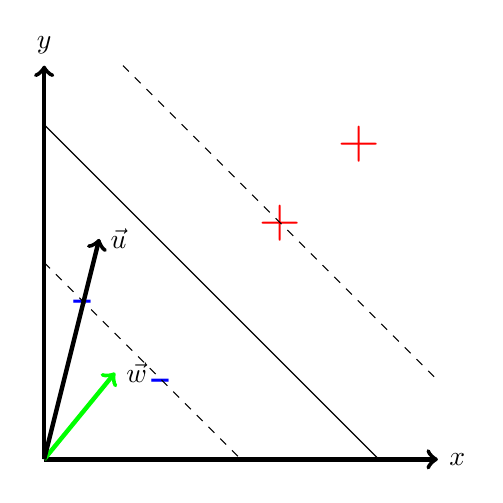
\begin{tikzpicture}


\draw[->,ultra thick] (0,0)--(5,0) node[right]{$x$};
\draw[->,ultra thick] (0,0)--(0,5) node[above]{$y$};

\node [text=blue] at (1.5,1) {\Huge -};
\node [text=blue] at (0.5,2) {\Huge -};
\node [text=red] at (3,3) {\huge +};
\node [text=red] at (4,4) {\huge +};



\draw[dashed]  (1,5)--(5,1);
\draw[dashed]  (0,2.5)--(2.5,0);
\draw(0,4.25)--(4.25,0);



\draw[->, ultra thick, green] (0,0)--(0.9,1.1) node[text=black, right]{$\vec{w}$};
\draw[->, ultra thick, black] (0,0)--(0.7,2.8) node[text=black, right]{$\vec{u}$};


\end{tikzpicture}
	\caption{Unknown sample vector.}
	\label{fig:fig6}
\end{figure}

If we take $\vec{w}$ and project a positive sample onto it

\begin{equation}
\label{eqn:pos_sample}
\vec{w}.\vec{x}_{+} + b \geq 1
\end{equation}

likewise

\begin{equation}
\label{eqn:neg_sample}
\vec{w}.\vec{x}_{-} + b \leq -1
\end{equation}


\begin{figure}[h]
	\centering
	\usetikzlibrary{arrows}
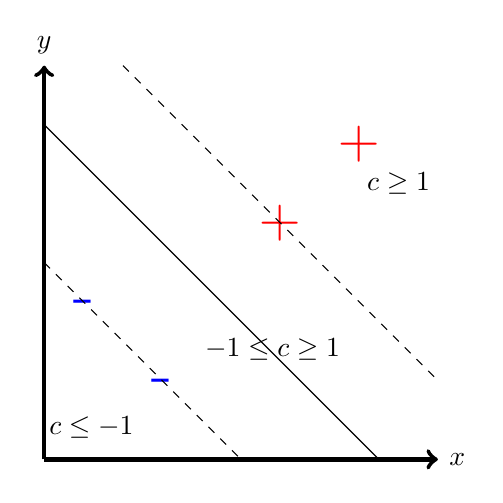
\begin{tikzpicture}


\draw[->,ultra thick] (0,0)--(5,0) node[right]{$x$};
\draw[->,ultra thick] (0,0)--(0,5) node[above]{$y$};

\node [text=blue] at (1.5,1) {\Huge -};
\node [text=blue] at (0.5,2) {\Huge -};
\node [text=red] at (3,3) {\huge +};
\node [text=red] at (4,4) {\huge +};



\draw[dashed]  (1,5)--(5,1);
\draw[dashed]  (0,2.5)--(2.5,0);
\draw(0,4.25)--(4.25,0);


\node at (4.5,3.5) {$c \geq 1$};
\node at (0.6,0.4) {$c \leq -1$};
\node at (2.9,1.4) {$ -1 \leq c \geq 1$};

\end{tikzpicture}

	\caption{Values of $c$ on the plane.}
	\label{fig:fig7}
\end{figure}


Introducing variable $y_i$ such that

\begin{tabular}{ll}
	$y_i$ & +1 for positive samples \\
	$y_i$ & -1 for negative samples \\
\end{tabular}

\bigskip
so equation (\ref{eqn:pos_sample}) becomes

\[
\vec{w}.\vec{x}_{i} + b \geq -1
\]
\[
(\vec{w}.\vec{x}_{i} + b) -1 \geq 0
\]
\[
y_i(\vec{w}.\vec{x}_{i} + b)-1 \geq 0
\]

for positive samples, and equation (\ref{eqn:neg_sample}) becomes

\[
\vec{w}.\vec{x}_{i} + b \leq -1
\]
\[
(\vec{w}.\vec{x}_{i} + b)  + 1 \leq 0
\]
\[
y_i(\vec{w}.\vec{x}_{i} + b)+1 \leq 0
\]
\[
y_i(\vec{w}.\vec{x}_{i} + b)-1 \geq 0
\]

for negative samples. 

Therefore we can conclude that

\begin{equation}
\label{eqn:constraint_outside_border}
y_i(\vec{w}.\vec{x}_{i} + b)-1 \geq 0
\end{equation}

we also define an additional constraint that 

\begin{equation}
\label{eqn:constraint_on_border}
y_i(\vec{w}.\vec{x}_{i} + b)-1 = 0
\end{equation}

for the values exactly on the boundary lines. Vectors to these values are termed as support vectors.

\bigskip

Equations (\ref{eqn:constraint_outside_border}) and (\eqref{eqn:constraint_on_border}) define the constraints for this system.


It is of particular interest to determine the distance between the boundaries. Consider a positive sample $x_{+}$ on the positive boundary with a vector $\vec{x}_{+}$ to it. Similarly, consider a negative sample $x_{-}$ on the negative boundary with a vector $\vec{x}_{-}$ to it. The width of the boundary can be found if we find the dot product of $x_{+} - x_{-}$ with a unit vector normal to the boundaries ($\frac{w}{\mid\mid w\mid\mid}$). Therefore the width, which is the scalar distance can be found by:

\begin{equation}
\label{eqn:width}
width = (\vec{x}_{+} - \vec{x}_{-}) . \frac{\vec{w}}{\mid\mid \vec{w} \mid\mid}
\end{equation}

but samples on the boundary are constrained by 

\[
y_i(\vec{w}.\vec{x}_{i} + b)-1 = 0
\]

where $y_i=1$ on the boundary. In this case, for the positive sample

\[
\vec{w}.\vec{x}_{+} = 1-b
\]

and for the negative sample

\[
-1(-\vec{w}.\vec{x}_{-} + b) = -1
\]
\[
-\vec{w}.\vec{x}_{-} - b -1 = 0
\]
\[
\vec{w}.\vec{x}_{-} = 1-b
\]

substituting in equation(\ref{eqn:width})


\begin{equation}
width = \frac{(1-b)-(1+b)}{\mid\mid \vec{w} \mid\mid} = \frac{2}{\mid\mid \vec{w} \mid\mid}
\end{equation}

The objective is to maximize the width, or maximize $\frac{2}{\mid\mid \vec{w} \mid\mid}$ or maximize $\frac{1}{\mid\mid \vec{w} \mid\mid}$ or minimize $\mid\mid w \mid\mid$ or minimize $ \frac{1}{2} \mid\mid \vec{w} \mid\mid^2$ under the constraints stated in equation(\ref{eqn:constraint_on_border}) and (\ref{eqn:constraint_outside_border}).


If we use Lagrange multipliers,


\begin{equation}
\label{eqn:svm_lagrange}
\mathcal{L}(w,b) = \frac{1}{2} \mid\mid \vec{w} \mid\mid^2 - \sum_{i} \lambda_{i}  y_i \left[ (\vec{w}_i \vec{x}_i +b ) -1 \right] 
\end{equation}

In this case, most constraint multipliers, $\lambda_{i}$ will be zero unless they are connected with vectors that lie on the boundary lines. Since we are dealing with $\mid\mid \vec{w} \mid\mid^2$ this type of optimization problem is referred to as a quadratic optimization one. One should note that the objective of this exercise is to minimize $w$ and maximize $b$, keeping in mind that the equation of the divisor hyperplane is $(\vec{w}.\vec{x})+b$.


\bigskip

From Lagrange Multiplier theory, the extremes can be found by using $\bigtriangledown \mathcal{L} =0$. 


\[
\frac{\partial \mathcal{L}}{\partial \vec{w}} = \vec{w} - \sum_{i} \lambda_{i} y_{i} \vec{x}_{i} = 0
\]

hence

\begin{equation}
\label{eqn:w_linear}
\vec{w} = \sum_{i} \lambda_{i} y_{i} \vec{x}_{i}
\end{equation}

It can be concluded from this equation that vector $\vec{w}$  is the linear sum of some of samples in the set, since for the other samples the value of $\lambda_{i}$ is zero, as stated before.


\[
\frac{\partial \mathcal{L}}{\partial b} = - \sum_{i} \lambda_{i} y_{i}  = 0
\]

that is

\begin{equation}
\label{eqn:lambda_y_0}
\sum_{i} \lambda_{i} y_{i}  = 0
\end{equation}

Substituting equation(\ref{eqn:w_linear}) in (\ref{eqn:svm_lagrange}) we get

\[
\mathcal{L} = \frac{1}{2} \sum_{i}\lambda_{i} y_{i}  \vec{x}_{i} \sum_{j}\lambda_{j} y_{j}\vec{x}_{j}  - \sum_{i}\lambda_{i} y_{i}  \vec{x}_{i} . \sum_{j}\lambda_{j} y_{j}\vec{x}_{j} - \sum_{i}\lambda_{i} y_{i} b + \sum_{i}\lambda_{i} 
\]

Consider the term $\sum_{i}\lambda_{i} y_{i} b $. This can be rewritten as $b\sum_{i}\lambda_{i} y_{i}$ since b is a constant. Form equation (\ref{eqn:lambda_y_0}), this term is 0.


Therefore,

\begin{equation}
\mathcal{L} = \sum_{i}\lambda_{i} - \frac{1}{2} \sum_{i}\sum_{j} \lambda_{i}\lambda_{j} y_{i} y_{j} \vec{x}_{i}.\vec{x}_{j}
\end{equation}

The maximum of this equation depends only on the dot product of pairs of samples. The decision rule, equation (\ref{eqn:decision_rule}) becomes;

\begin{equation}
\sum_{i} \lambda_{i} y_{i} \vec{x}_{i} . \vec{u} + b \geq 0 \implies positive
\end{equation}

The decision rule depends on the dot product of the unknown and the other samples.

If the samples are not linearly separable, a different perspective is taken by applying a transformation, $\phi(x)$

\begin{figure}[h]
	\centering
	\usetikzlibrary{arrows}
\begin{tikzpicture}

\draw[->] (0,0)--(5,0) node[right]{$x$};
\draw[->] (0,0)--(0,5) node[above]{$y$};

\node [text=blue] at (2,2) {\Huge -};
\node [text=blue] at (0,0) {\Huge -};
\node [text=red] at (2,0) {\huge +};
\node [text=red] at (0,2) {\huge +};

\draw[->] (0,-6)--(5,-6) node[right]{$x$};
\draw[->] (0,-6)--(0,-1) node[above]{$y$};
\draw[->] (0,-6)--(3,-3) node[above]{$z$};

\draw[dashed, gray] (1.5,-4.5)--(4,-4.5);
\draw[dashed, gray] (4,-4.5)--(2.5,-6);
\draw[dashed, gray] (4,-4.5)--(4,-3);
\draw[dashed, gray] (4,-3)--(1.5,-3);
\draw[dashed, gray] (1.5,-4.5)--(1.5,-3);
\draw[dashed, gray] (2.5,-4.5)--(2.5,-6);
\draw[dashed, gray] (2.5,-4.5)--(4,-3);

\node [text=red] at (1.5,-3) {\huge +};
\node [text=red] at (2.5,-4.5) {\huge +};
\node [text=blue] at (4,-4.5) {\Huge -};
\node [text=blue] at (0,-6) {\Huge -};

\node at (2.5,3) {linearly inseparable samples};
\node at (2.5,-2) {separable after transformation};

\end{tikzpicture}
	\caption{Resolution of linearly inseparable samples.}
	\label{fig:fig8}
\end{figure}
 
As was discussed previously, the maximization depends on the dot product of the samples. Hence, by applying the mentioned transformation, maximization now depends on

\[
\phi(\vec{x}_{i}) . \phi(\vec{x}_{j})
\]

Using the same reasoning the decision becomes dependent on

\[
\phi(\vec{x}_{i}) . \phi(\vec{u})
\]

Hence the function will be necessary,

\begin{equation}
\label{eqn:kernel}
K(\vec{x}_{i}, \vec{x}_{j}) = \phi(\vec{x}_{i}) . \phi(\vec{x}_{j})
\end{equation}

Function K is called the kernel and provides the dot product of the two vectors in another space.

\subsubsection{Linear Kernel}

\begin{equation}
\label{eqn:kernel_linear}
K(\vec{x}_{i}, \vec{x}_{j}) = (\vec{x}_{i}. \vec{x}_{j} + 1) ^n
\end{equation}


\subsubsection{Radial Basis}

\begin{equation}
\label{eqn:kernel_radial}
K(\vec{x}_{i}, \vec{x}_{j}) = e^{(\frac{\mid\mid \vec{x}_{i} - \vec{x}_{j}  \mid\mid}{\sigma})}
\end{equation}

If $\sigma$ is very small over-fitting will take place

\end{document}
